% This is samplepaper.tex, a sample chapter demonstrating the
% LLNCS macro package for Springer Computer Science proceedings;
% Version 2.21 of 2022/01/12
%
\documentclass[runningheads]{llncs}
%
\usepackage[T1]{fontenc}
% T1 fonts will be used to generate the final print and online PDFs,
% so please use T1 fonts in your manuscript whenever possible.
% Other font encondings may result in incorrect characters.
%
\usepackage{booktabs}
\usepackage{graphicx}
\usepackage{tikz}
\usepackage{float}
\usepackage{longtable}
\usepackage{adjustbox}

\usetikzlibrary{positioning}
% Used for displaying a sample figure. If possible, figure files should
% be included in EPS format.
%
% If you use the hyperref package, please uncomment the following two lines
% to display URLs in blue roman font according to Springer's eBook style:
%\usepackage{color}
%\renewcommand\UrlFont{\color{blue}\rmfamily}
%\urlstyle{rm}
%
\begin{document}
%
\title{Knowledge Graph Reengineering Along the Ontological Continuum}
%
%\titlerunning{Abbreviated paper title}
% If the paper title is too long for the running head, you can set
% an abbreviated paper title here
%
\author{First Author\inst{1}\orcidID{0000-1111-2222-3333} \and
Second Author\inst{2,3}\orcidID{1111-2222-3333-4444} \and
Third Author\inst{3}\orcidID{2222--3333-4444-5555}}
%
\authorrunning{F. Author et al.}
% First names are abbreviated in the running head.
% If there are more than two authors, 'et al.' is used.
%
\institute{Princeton University, Princeton NJ 08544, USA \and
Springer Heidelberg, Tiergartenstr. 17, 69121 Heidelberg, Germany
\email{lncs@springer.com}\\
\url{http://www.springer.com/gp/computer-science/lncs} \and
ABC Institute, Rupert-Karls-University Heidelberg, Heidelberg, Germany\\
\email{\{abc,lncs\}@uni-heidelberg.de}}
%
\maketitle              % typeset the header of the contribution
%
\begin{abstract}
Knowledge graphs have become the primary vehicle for data integration and are critical to the success of modern AI --- but the diversity of KG modelling practices, from lightweight vocabularies to richly axiomatised ontologies, makes integration and reuse expensive and brittle. This challenge is particularly acute in neuro-symbolic AI, where bridging neural and symbolic components depends on the ability to reengineer KGs to fit new requirements; GenAI now offers unprecedented automation capability, but without a principled understanding of the KG space, such automation remains conceptually ungrounded. We introduce the ontological continuum as that missing conceptualisation --- a structured representational space organised around two axes: semantics $\leftrightarrow$ pragmatics, and properties $\leftrightarrow$ affordances; together these define a vocabulary to describe, compare, navigate, and transform KGs across the spectrum. The methodological stance is empirical: rather than prescribing how KGs should be modelled, the continuum aims to be a theory of the existent --- derived from observation of real-world KG engineering practices --- marking a shift from knowledge engineering as a design science to knowledge engineering as an empirical one. We ground the vision through a case study on provenance knowledge, showing how a single concern manifests differently across the spectrum and how transformations between positions can be characterised and automated. We articulate four open research challenges and invite the community to develop the ontological continuum as a shared research agenda.
\keywords{Knowledge Graph Reengineering \and Ontological Continuum \and Affordances \and Neuro-Symbolic AI \and Empirical Knowledge Engineering}
\end{abstract}



%
%
%
\section{Introduction}

\begin{itemize}
    \item KGs have become the primary vehicle for data integration and are critical to trustworthy AI.
    \item Neuro-symbolic AI needs agile, transformable KG content to bridge neural and symbolic components.
    \item GenAI and LLMs offer unprecedented capability to automate KG reengineering tasks --- enabling agents that can reason step-by-step through reengineering decisions with a degree of autonomy. % [NEW]
    \item This agentic turn is already underway: emerging work on autonomous knowledge engineering agents --- systems that decompose, plan, and execute KG engineering tasks with minimal human intervention --- makes the absence of a principled map of the KG space particularly acute. An agent navigating reengineering decisions without such a map is forced to treat the KG ecosystem as an undifferentiated black box, with no principled basis for choosing transformations, estimating their cost, or explaining its choices. % [NEW]
	\item Yet both forces operate without a principled understanding of the space they are navigating.
    \item The KG ecosystem is diverse by nature, and this diversity is healthy --- but it comes at a cost: adapting content is still an expensive and difficult task.
    \item The dominant response has been structural harmonisation — thirty years of mapping, aligning, and merging — yet cross-KG reuse remains expensive and brittle in practice. The right question is not "how similar is KG A to KG B?" but "does KG A afford what community C needs for task T?" — a question current approaches, and their quality metrics, entirely miss. % [NEW]
    \item What is missing is a flexible and comprehensive conceptualisation of how diverse modelling practices interplay --- one that integrates both the semantic dimension (domain meanings) and the pragmatic dimension (what a KG affords to whom, for which task). % [NEW]
    %\item Work such as Fa\c{c}ade-X already demonstrates what a pragmatics-aware approach looks like in practice; what is missing is the overarching conceptualisation that generalises and grounds such approaches. % [NEW]
    %This direction is gaining traction beyond individual tools: the W3C Data Façades Community Group is actively developing standards in this space, signalling that pragmatics-aware KG access is becoming a community-level concern.
	\item We introduce the ontological continuum as that missing conceptualisation.
	\item The contribution of this paper is conceptual and terminological: we define the meta-model of the continuum along its semantic and pragmatic dimensions, as a foundation for a theory to be developed by the community, and we propose the vocabulary to describe positions within it and the transformations between them. We use the term \emph{continuum} in a conceptual, not a mathematical sense: it is not a space that exists a priori, populated by infinitely many independent points, but one that is constructed for a specific operational need --- derived empirically from representative KGs, and organised through the relationships among their observable properties and affordances. % [NEW]
    \item We call on the community to develop it as a shared research agenda.
\end{itemize}

\section{Background and Related Work}

The KG ecosystem is rich and diverse --- from lightweight vocabularies to richly axiomatised ontologies --- and this diversity is both healthy and necessary. Yet it comes at a cost.

\begin{itemize}
    \item The KG ecosystem spans from lightweight vocabularies (Dublin Core, Schema.org) to richly axiomatised ontologies (Gene Ontology, SNOMED CT).
    \item Different communities have developed different formalisms, governance practices, and modelling methodologies, each fit for purpose.
    \item \textit{Knowledge and ontology engineering:} methodologies (NeOn, LOT, MOMO) provide guidance but assume a one-size-fits-all approach; reuse practices are poorly understood and underspecified. Diversity runs deeper than formalisms: foundational ontology choices --- BFO, DOLCE, UFO --- create incompatibilities at the level of the conceptual model, with real downstream consequences. For example, antipatterns defined within a UFO-based validation framework cannot be straightforwardly applied in a DOLCE-based setting; bridging them requires explicit mappings, operationalised as SPARQL negative competency questions --- a form of ad hoc pragmatic adaptation that the field currently has no principled framework to support. % [NEW]
	\item \textit{KG construction, interoperability, and alignment:} mapping languages (R2RML, RML), ontology alignment systems (LogMap, AML), and modularisation techniques enable integration but fall short of addressing diversity in a unified way. A further blind spot is the implicit assumption that alignment must be complete: evaluation benchmarks and quality metrics consistently reward full coverage, yet fit-for-purpose reuse requires only the fragments relevant to a given task --- not a complete mapping to a target schema. The continuum makes this distinction explicit, replacing completeness as a quality criterion with task-relative coverage. % [NEW]
    \item \textit{A methodological precedent:} Fa\c{c}ade-X~\cite{facadex} derives a unified access mechanism for heterogeneous, non-RDF data sources through empirical analysis of their structural characteristics, enabling SPARQL querying without schema harmonisation. The move is bottom-up and observation-first: rather than prescribing how sources should be structured, it characterises what they afford and builds the framework from there. The ontological continuum adopts the same methodological stance, extending it from the narrow question of query affordances over heterogeneous data sources to the full space of KG modelling practices. That this direction is gaining traction beyond individual tools is signalled by the W3C Data Fa\c{c}ades Community Group, which is actively developing standards in this space.
	\item \textit{Partial pragmatic predecessors:} pay-as-you-go approaches and ontology modularisation have partially addressed the question of fit-for-purpose reuse, but without an explicit affordance framing --- they remain task-agnostic and community-agnostic. % [NEW]
    \item \textit{GenAI and LLMs for KE:} a growing body of work --- including systematic surveys --- applies LLMs to ontology design, competency question engineering, SPARQL generation, and schema induction; powerful, but all sharing the same blind spot: they operate without a principled model of the KG space they are navigating. % [NEW]
    \item \textit{A cautionary precedent:} semantic web services (OWL-S and related work) modelled the semantic layer well but left the pragmatic layer --- how resources are composed and used in practice --- unaddressed; the initiative collapsed under that weight, a lesson that neglecting pragmatics has real consequences. % [NEW]
    The risk is not merely historical: one might assume that GenAI now finally delivers the autonomy that semantic web services promised — but without a principled pragmatic framework, the same failure mode applies.
    \item \textit{The affordance framing as a missing lens:} the philosophical literature on affordances (Gibson, Norman) has been extensively applied in HCI and design, but has barely touched KG engineering; bringing it in provides a principled way to talk about use-relative KG properties --- what a KG affords to whom, for which task. % [NEW]
    \item The gap is not a missing technique but a missing conceptualisation: no existing framework offers a principled, dimension-aware account of how diverse modelling practices interplay --- leaving both neuro-symbolic integration and GenAI-driven automation conceptually ungrounded. % [NEW]
\end{itemize}

\section{The Ontological Continuum: A Vision}

\begin{itemize}
    \item The ontological continuum is organised around two axes: semantics $\leftrightarrow$ pragmatics, and properties $\leftrightarrow$ affordances; together these define a 2$\times$2 conceptual space that is the core vocabulary of the framework. % [NEW]
    \item \textit{Semantic properties} capture meanings relevant to domains of interest; \textit{semantic affordances} capture meanings applicable to specific downstream tasks and communities --- what a KG means is inseparable from what it is used for. % [NEW]
    \item \textit{Pragmatic properties} capture the meta-models used to represent statements (RDF, OWL, RDF-Star, Wikidata model); \textit{pragmatic affordances} capture specific ways of exploiting those meta-models in practice --- for example, efficient path traversal or aggregation queries in SPARQL, class subsumption or property chain inference in OWL, constraint validation in SHACL, or reification patterns in RDF-Star. % [NEW]
    %\item These four categories are not independent: a semantic commitment shapes which pragmatic affordances are available, and a pragmatic choice constrains what semantic properties can be expressed; the continuum makes these dependencies explicit. % [NEW]
	\item These four categories are not independent: a semantic commitment shapes which pragmatic affordances are available, and a pragmatic choice constrains what semantic properties can be expressed. For example, if the required semantic affordance is attribution, this determines which pragmatic properties must be present in the KG to support it; conversely, choosing RDF-Star as a pragmatic property opens certain SPARQL affordances while foreclosing others. The continuum makes these dependencies explicit --- and formalising them, including the directionality and transitivity of cross-dimension constraints, is itself a core research challenge for the community to address. % [NEW]
    \item A key ambition of the continuum is to replace the blurred notion of ``community'' with a formal set of dimensions: rather than saying a KG is fit for a given community, we can say it exhibits a specific combination of semantic and pragmatic properties and affordances --- making fitness for purpose operational and measurable. % [NEW]
%    \item The 2$\times$2 space is a starting generalisation; the concrete properties and affordances that populate each quadrant are not assumed but derived --- through empirical analysis of real-world KGs, downstream applications, and community practices. % [NEW]
    \item The 2$\times$2 space is a starting generalisation; the concrete properties and affordances that populate each quadrant are not assumed but derived --- through empirical analysis of real-world KGs, downstream applications, and community practices. The methodology is iterative: representative KGs are analysed one by one, keywords are assigned per dimension, existing terms are reused wherever possible, and new ones are introduced only when necessary --- with retrospective verification across previously analysed KGs to ensure consistency. The resulting keyword-attribute matrix can then be projected into a mathematically ordered space: Formal Concept Analysis (FCA) is one well-suited choice, producing a concept lattice that gives the continuum its ordered structure; other projections are possible and may be preferable depending on the task. % [NEW]
	\item The methodological stance is descriptive: the continuum aims to be a theory of the existent --- of what KG engineering practices are --- rather than a normative theory of what they should be; this distinguishes it from prescriptive methodology work and upper ontology efforts. % [NEW]
    \item The continuum does not prescribe a single modelling approach --- it provides a vocabulary to describe, compare, navigate, and transform KGs across the spectrum.
    \item Transformations along the continuum are characterised explicitly by what they cost and what they lose: some are lossless, some reduce expressivity, some require augmenting knowledge; making this explicit is what distinguishes principled reengineering from ad hoc adaptation. % [NEW]
    \item The continuum enables GenAI agents to navigate reengineering decisions step-by-step, exploring dimensions autonomously --- in the limit, given only a characterisation of input and output, an agent can identify and perform the right transformations without human intervention. % [NEW]
    \item It also enables neuro-symbolic systems to identify and perform the right transformations when integrating KGs with different commitments.
\end{itemize}

\section{A Case Study: Provenance Knowledge Across the Continuum}

\begin{itemize}
    \item Three scenarios illustrate the relevance of the continuum across different contexts: (1) bioinformatics, where richly axiomatised ontologies (Gene Ontology, SNOMED CT, OBO Foundry) with strong realist commitments must interoperate with more lightweight or provisional representations; (2) cultural heritage, where overlapping publication standards (Linked Art, EODEM, CIDOC-CRM) apply to the same collections data and no full harmonisation is feasible; (3) provenance, where a single concern manifests very differently across the spectrum. % [NEW]
    \item We zoom into provenance as the worked example: it is the right choice because provenance models are genuinely diverse --- ranging from a single property (\texttt{dc:source}) to full ontological modelling (PROV-O) --- whereas process knowledge models are comparatively homogeneous. % [NEW]
    \item We analyse 3--5 concrete provenance models --- Dublin Core (\texttt{dc:source}), named graphs, RDF-Star reification, PROV-O, and Wikidata qualifiers/truthy statements --- each occupying a different position in the continuum. % [NEW]
    \item For each model, we characterise its position in the 2$\times$2 space: what semantic properties and affordances it offers, and what pragmatic properties and affordances it supports --- making the abstract framework concrete. % [NEW]
    \item We show how the continuum captures these variations as positions along its dimensions.
    \item We illustrate how transformations between these positions can be described and, ultimately, automated --- making explicit what is lost or gained at each step: for example, moving from \texttt{dc:source} to PROV-O enriches semantic properties but increases pragmatic complexity; moving from PROV-O to Wikidata qualifiers trades expressive power for a different set of pragmatic affordances. % [NEW]
    \item The case study demonstrates the practical value of the continuum and its relevance to real-world KG engineering challenges.
\end{itemize}

Methodology for populating the continuum:

The following procedure is presented not as a definitive taxonomy of provenance approaches, but as a demonstration that the dimensions of the ontological continuum can be characterised empirically --- that existing KGs can be positioned within this space, and that the resulting structure, when projected through FCA or similar techniques, yields a principled ordering. The keywords and attributes produced are illustrative; a different analyst, or a different task, would produce a different but equally valid instantiation of the continuum.

\begin{enumerate}
    \item Select a set of real-world KGs of interest, each representing a distinct approach to the concern under study (here: provenance).
    \item Define the four dimensions of the ontological continuum: semantic properties, semantic affordances, pragmatic properties, and pragmatic affordances.
    \item For each dimension, provide a contextualised definition grounded in the concern under study.
    \item For each KG, populate each dimension with a list of keywords, one KG at a time, reviewing the output before moving to the next.
    \item Reuse existing keywords whenever possible; introduce new keywords only when necessary.
    \item When a new keyword is introduced, define it explicitly if its meaning is not obvious.
    \item When a new keyword is introduced, verify retrospectively whether it applies to previously analysed KGs, and update those if necessary.
    \item Review the full keyword lists periodically to harmonise terminology --- collapsing synonyms, resolving ambiguities, and ensuring consistency across KGs.
    \item Produce the final keyword lists as \texttt{KG,keyword} pairs, one per dimension, ready for further analysis and visualisation.
\end{enumerate}

Open questions:

What are the dependencies across the attributes in each dimension (sem prop <-> sem aff, sem prop <-> prag prop, etc...)?


\subsection{Zooming into provenance}

\begin{itemize}
    \item \textbf{Simple metadata annotations}: Dublin Core terms such as \texttt{dc:creator} and \texttt{dc:date} are widely used to attach provenance metadata at the dataset or document level, as in DBpedia dataset descriptions~\cite{dcterms}.
    \item \textbf{Named graphs}: Provenance metadata can be associated with sets of triples by grouping them into named graphs, as adopted in Wikidata to attach references to groups of statements~\cite{wikidata}.
    \item \textbf{RDF reification}: The standard RDF reification vocabulary (\texttt{rdf:Statement}) allows metadata to be attached to individual triples, and was widely used in early Linked Data deployments~\cite{rdf11}.
    \item \textbf{RDF-Star}: A more compact mechanism for annotating individual triples by embedding a triple as the subject of another triple, now gaining adoption in newer KG deployments~\cite{rdfstar}.
    \item \textbf{Wikidata model}: A bespoke meta-model using qualifiers and references attached to statements, representing a community-driven pragmatic solution distinct from standard RDF mechanisms~\cite{wikidata}.
    \item \textbf{PROV-O}: A full ontological model of provenance, capturing agents, activities, entities and their relationships, adopted in scientific workflows and open science practices~\cite{provo}.
    \item \textbf{Schema.org markup}: A lightweight, web-scale vocabulary used to annotate entities and datasets with provenance metadata such as source, creator, and licence, as adopted by Google Data Commons, which extends Schema.org to attach a provenance property to every triple in the graph~\cite{datacommons,schemaorg}.
\end{itemize}

Ontological continuum dimensions in context:

\begin{itemize}
    \item \textbf{Semantic properties}: What provenance meaning is captured --- e.g.\ authorship, temporal information, lineage, trust, process descriptions.
    \item \textbf{Semantic affordances}: What downstream tasks the provenance representation supports --- e.g.\ trust assessment, data quality evaluation, reproducibility, audit trails, attribution.
    \item \textbf{Pragmatic properties}: The representational mechanism used --- simple metadata annotations, named graphs, RDF reification, RDF-Star, Wikidata model, PROV-O.
    \item \textbf{Pragmatic affordances}: What interaction methods are supported --- e.g.\ SPARQL querying, SHACL validation, OWL reasoning.
\end{itemize}

Examples for each approach:

\begin{itemize}
    \item \textbf{Europeana} uses the Europeana Data Model (EDM), which captures provenance through OAI-ORE Aggregations, recording the original data provider, intermediaries, and Europeana itself as aggregator, with Dublin Core elements at the core of the descriptive metadata~\cite{haslhofer2011}.
    \item \textbf{Google Data Commons} extends the Schema.org vocabulary to attach a provenance property to every triple in the graph, recording the URL of the originating data provider as a first-class element of the data model~\cite{datacommons,schemaorg}.
    \item \textbf{Bio2RDF} stores provenance metadata for each dataset in a dedicated named graph per SPARQL endpoint, using VoID, PROV, and Dublin Core to describe the date of conversion, licensing, and the script used to generate the dataset~\cite{callahan2013}.
    \item \textbf{The British Museum ResearchSpace} platform uses RDF reification patterns grounded in the CIDOC Conceptual Reference Model (CRM) to capture the provenance of scholarly assertions about cultural heritage objects~\cite{researchspace}.
    \item \textbf{UniProt} has adopted RDF-Star as a more compact and performant mechanism for attaching evidence and provenance annotations to individual triples in the knowledgebase, replacing a verbose and costly reification-based approach~\cite{rdfstar,uniprot}.
    \item \textbf{Wikidata} uses a bespoke statement model in which every claim can be qualified and referenced using a dedicated meta-model of statements, qualifiers, and references, providing fine-grained provenance at the level of individual assertions~\cite{vrandevcic2014,hernandez2015}.
    \item \textbf{The European Union Open Data Portal} captures provenance of published datasets through the DCAT Application Profile (DCAT-AP), which incorporates PROV-O via \texttt{prov:qualifiedAttribution} to express agent roles and data lineage~\cite{provo,dcatap}.
    \item \textbf{DBpedia} organises its extracted Wikipedia data into named graphs per language and dataset, using PROV-O to record dataset-level provenance metadata including the extraction process and the originating source~\cite{dbpedia}.
    \item \textbf{Linked Open Vocabularies (LOV)} tracks the provenance of vocabulary publications and their dependencies using PROV-O, recording authors, publishers, versioning history, and the agents responsible for curation within the vocabulary ecosystem~\cite{lov}.
    \item \textbf{Nanopublications} treat provenance as a first-class structural concern: each nanopublication consists of three named graphs --- assertion, provenance, and publication info --- with PROV-O used within the provenance graph to capture authorship, temporal information, and the epistemic status of scientific claims~\cite{nanopub}.
\end{itemize}


\section{Discussion}

TBD

\section{Research Challenges for the Community}

\begin{itemize}
    \item \textbf{Challenge 1:} Characterising and formalising the dimensions of diversity in KG modelling practices --- what are the relevant dimensions, and how can they be operationalised?
    \begin{itemize}
        \item Deriving the concrete semantic and pragmatic properties and affordances that populate the 2$\times$2 space, through empirical analysis of real-world KGs and community practices. % [NEW]
        \item Defining community-relative fitness metrics: given a task, what combination of dimensions does a KG need to exhibit, and how can this be measured precisely? % [NEW]
        \item Replacing the informal notion of ``community'' with a formal, operational characterisation in terms of continuum dimensions. % [NEW]
    \end{itemize}
	\item \textbf{Challenge 2:} Formalising the dependencies between continuum dimensions --- how do choices in one dimension constrain or determine options in others?
    \begin{itemize}
        \item Identifying the directionality and transitivity of cross-dimension constraints: for example, which semantic affordances entail specific pragmatic properties, and which pragmatic choices foreclose certain semantic commitments. % [NEW]
        \item Developing a formal account of these dependencies that can be used to guide transformations --- so that when a target affordance is specified, the required properties in all four dimensions can be derived systematically. % [NEW]
        \item Understanding how foundational ontology choices (BFO, DOLCE, UFO) propagate through the dimensions: an upper-level commitment is not merely a semantic property but one that cascades into pragmatic affordances, validation strategies, and alignment compatibility. % [NEW]
    \end{itemize}
	
    \item \textbf{Challenge 3:} Enabling modular, context-aware reuse across the spectrum --- how can ontological fragments be extracted, aligned, and applied across KGs with different commitments?
    \begin{itemize}
        \item Developing adaptive query mechanisms that are dimension-aware --- translating user intent into KG-specific queries without requiring schema alignment, taking into account the semantic and pragmatic constraints imposed by each KG. % [NEW]
        \item Estimating the cost of adaptation: what is lost at each transformation step, what effort is required to bring a KG to the affordance level a task requires, and how can this be made explicit and manageable? % [NEW]
    \end{itemize}

    \item \textbf{Challenge 4:} Supporting the co-evolution of interdependent KG engineering artefacts --- how do changes in one artefact (schema, mapping, query, documentation) propagate across the ecosystem?
    \begin{itemize}
        \item Developing a ``What if'' analysis framework: for every semantic choice, making the pragmatic consequences explicit, and vice versa --- so that design decisions are informed by their downstream effects across the continuum. % [NEW]
    \end{itemize}
	
	\item \textbf{Challenge 5:} Developing human-in-the-loop strategies that make reengineering accessible to users with varying expertise --- how can GenAI reduce cognitive load while maintaining quality?
	    \begin{itemize}
	        \item Deriving implications for KG engineering practice from the affordance framing: if pragmatics comes first, how should KGs be designed, published, and maintained so that their affordances are explicit and reusable? % [NEW]
	        \item Supporting bidirectional design: helping users navigate the trade-offs between semantic expressivity and pragmatic accessibility, with GenAI acting as an informed guide through the continuum. % [NEW]
	        \item Supporting agentic KE: as autonomous agents begin to perform KE tasks with some degree of discretion, the continuum provides the reference framework they need to make reengineering decisions that are not merely executable but explainable --- every transformation choice can be grounded in continuum dimensions, its cost made explicit, and its provenance recorded. Without such a framework, agent decisions remain opaque, undermining trust and making troubleshooting impossible. % [NEW]
	    \end{itemize}
\end{itemize}

\section{Conclusion}

\begin{itemize}
    \item The ontological continuum is the missing conceptualisation for principled KG reengineering --- its concrete contribution is terminological: a vocabulary and meta-model, organised around the axes of semantics $\leftrightarrow$ pragmatics and properties $\leftrightarrow$ affordances, that the community can build on. % [NEW]
    \item The timing is right: GenAI offers the automation capability; neuro-symbolic AI creates the demand --- and the vision of autonomous agents navigating reengineering decisions along the continuum is now within reach. % [NEW]
    \item The continuum embodies a deeper reframing of knowledge engineering research culture: from a design science that prescribes what KG artefacts should be, to an empirical science that observes what they are --- deriving theory from the rich, diverse ecosystem of KGs that the web and the democratisation of computing have made available for the first time. % [NEW]
    \item This empirical turn is the opportunity of 2026: just as physics and biology build theories by observing natural phenomena, knowledge engineering can now build its theories on an empirical basis --- a theory of the existent rather than one of the possible. % [NEW]
    \item The community is invited to pursue this as a shared research agenda --- specifically: to populate the continuum empirically, to develop fitness metrics and adaptive mechanisms along the lines sketched in Section~\ref{sec:challenges}, and to validate the framework across diverse domains and communities. % [NEW]
    \item Achieving this requires collaboration across knowledge engineering, AI, and application domains --- and a willingness to let observations of real-world practice, rather than idealised design criteria, drive the theory. % [NEW]
\end{itemize}

%\section*{EKAW2026:  The Pragmatics-First Manifesto}

\subsection*{Core point}

KG reuse research has been obsessed with alignment  finding perfect correspondences between schemas. But real-world users don't need perfect alignment; they need good-enough access to knowledge they didn't build. This paper makes the case for a pragmatics-first approach to KG reuse: adapting queries to KGs rather than KGs to queries, and treating "fit for purpose" as a community-relative, task-dependent property rather than a universal standard.

\subsection*{Main Claim}

The dominant paradigm in KG reuse research assumes that interoperability requires structural harmonisation — mapping, aligning, or merging KG schemas. This paper argues this is the wrong goal. Real KG reuse is *pragmatic*: users have tasks, KGs have affordances, and the question is whether a KG's affordances are sufficient for the task — not whether it can be perfectly aligned with any other KG. This reframing suggests a different research agenda: characterising KG affordances, developing adaptive query mechanisms, and building tools that meet users where they are rather than requiring them to harmonise everything first.

\subsection*{What Makes It Original}

The philosophical literature on affordances (Gibson 1979; Norman 1988) has been applied extensively in HCI and design but barely touched KG engineering. Bringing this framing into the KG space provides a principled way to talk about *use-relative* properties — properties that depend on who is using the KG and for what — and to explain why the "one alignment to rule them all" approach has consistently underperformed in practice.

Crucially, this paper is not purely argumentative: the team has already built a working example of a pragmatics-first approach. Façade-X (Asprino, Daga, Gangemi \& Mulholland 2023) constructs *de facto* knowledge graphs over heterogeneous non-RDF data sources via SPARQL, without requiring the underlying data to be transformed or mapped to a common schema. This is exactly what pragmatics-first looks like in practice — meet users where their data already is, rather than requiring them to harmonise it first. Having a concrete published system as the paper's central motivating example significantly strengthens the argument and distinguishes it from a purely theoretical position paper.

\subsection*{Proposed Structure}

Section 1: The Alignment Imperative and Its Limits. The history of KG interoperability research as a series of attempts to achieve alignment: from DAML+OIL mappings through OWL ontology matching through current LLM-based alignment. Despite thirty years of effort and impressive technical progress, cross-KG reuse remains expensive and brittle in practice. Why?

Section 2: A Pragmatic Turn. Introduce the affordance framing: a KG's value is not intrinsic but relational,  it depends on what a user (or user community) needs it to do. This means the right question is not "how similar is KG A to KG B?" but "does KG A afford what community C needs for task T?" Survey how this question has been partially addressed in ontology engineering (e.g., pay-as-you-go approaches, ontology modularisation) and where it has not been addressed at all.

Section 3: A Pragmatics-First Approach in Practice. Ground the argument in concrete work. Façade-X [Asprino, Daga, Gangemi \& Mulholland 2023] is presented as the leading working example of a pragmatics-first tool: it enables SPARQL querying of heterogeneous, non-RDF data without schema harmonisation, generating *de facto* KGs whose characteristics are determined by the query needs of the user, not by the data's native structure. This section generalises from Façade-X to define semantic affordances (meanings relevant to specific domains), pragmatic affordances (interaction methods the KG supports), and — in brief — emerging agentic affordances (what AI agents can do with the KG without human mediation). The cultural heritage domain provides a second running example throughout: institutions such as museums hold rich legacy collections that need to be published as Linked Data under multiple overlapping standards (Linked Art, EODEM, CIDOC-CRM), a textbook case of where pragmatics-first tools are needed because no harmonisation is feasible. Note that characterising affordances requires describing the user community as well as the KG — a point current quality metrics entirely miss.

Section 4: What a Pragmatics-First Agenda Looks Like Sketch three research directions that follow from the affordance framing: (1) community-relative KG fitness metrics — how do we formally specify what a community needs a KG to afford?; (2) adaptive query mechanisms that translate user intent into KG-specific queries without requiring schema alignment, building on the façade and query rewriting tradition; (3) methods for estimating the cost of adaptation, how much effort is required to bring a KG to the affordance level a community needs? Each direction is illustrated with an open problem and a pointer to relevant existing work.

Section 5: Implications for KG Engineering Practice.
How does a pragmatics-first view change the way we should build, publish, and maintain KGs? Argue for affordance-driven KG design: build KGs with explicit documentation of what they afford to whom, rather than striving for universal reusability.




\begin{credits}
\subsubsection{\ackname} We thank.... Enrico: ClimateSense and MultiPod

% \subsubsection{\discintname} Conflicts
\end{credits}

%
% ---- Bibliography ----
%
% BibTeX users should specify bibliography style 'splncs04'.
% References will then be sorted and formatted in the correct style.
%
\clearpage
\bibliographystyle{splncs04}
\bibliography{main}
%

\section*{Appendix: Provenance in the Continuum}

\subsection*{Tables}
% Semantic properties of provenance across knowledge graphs.
\begin{table}[ht]
\centering
\small
\begin{tabular}{lccccccc}
\toprule
 & \rotatebox{90}{\textbf{Europeana}} & \rotatebox{90}{\textbf{Google Data Commons}} & \rotatebox{90}{\textbf{Bio2RDF}} & \rotatebox{90}{\textbf{British Museum ResearchSpace}} & \rotatebox{90}{\textbf{UniProt}} & \rotatebox{90}{\textbf{Wikidata}} & \rotatebox{90}{\textbf{EU ODP}} \\
\midrule
\textit{temporal information} &  &  & $\times$ & $\times$ & $\times$ & $\times$ & $\times$ \\
\textit{data provider} & $\times$ & $\times$ & $\times$ &  &  & $\times$ & $\times$ \\
\textit{authorship} & $\times$ &  &  & $\times$ & $\times$ & $\times$ & $\times$ \\
\textit{dataset-level lineage} & $\times$ & $\times$ & $\times$ &  &  &  & $\times$ \\
\textit{epistemic status} &  &  &  & $\times$ & $\times$ & $\times$ &  \\
\textit{triple-level lineage} &  & $\times$ &  &  & $\times$ & $\times$ &  \\
\textit{licensing} & $\times$ &  & $\times$ &  &  &  &  \\
\textit{evidence type} &  &  &  &  & $\times$ & $\times$ &  \\
\textit{aggregation chain} & $\times$ &  &  &  &  &  &  \\
\textit{agent roles} &  &  &  &  &  &  & $\times$ \\
\textit{conversion process} &  &  & $\times$ &  &  &  &  \\
\textit{source organisation} &  & $\times$ &  &  &  &  &  \\
\textit{scholarly assertion} &  &  &  & $\times$ &  &  &  \\
\bottomrule
\end{tabular}
\caption{Semantic properties of provenance across knowledge graphs.}
\label{tab:semantic_properties}
\end{table}

% Semantic affordances of provenance across knowledge graphs.
\begin{table}[ht]
\centering
\small
\begin{tabular}{lccccccc}
\toprule
 & \rotatebox{90}{\textbf{Europeana}} & \rotatebox{90}{\textbf{Google Data Commons}} & \rotatebox{90}{\textbf{Bio2RDF}} & \rotatebox{90}{\textbf{British Museum ResearchSpace}} & \rotatebox{90}{\textbf{UniProt}} & \rotatebox{90}{\textbf{Wikidata}} & \rotatebox{90}{\textbf{EU ODP}} \\
\midrule
\textit{attribution} & $\times$ & $\times$ & $\times$ & $\times$ & $\times$ & $\times$ & $\times$ \\
\textit{source tracking} &  & $\times$ & $\times$ & $\times$ & $\times$ & $\times$ &  \\
\textit{data discovery} & $\times$ & $\times$ & $\times$ &  &  &  & $\times$ \\
\textit{reproducibility} &  &  & $\times$ &  & $\times$ &  & $\times$ \\
\textit{rights management} & $\times$ &  & $\times$ &  &  &  & $\times$ \\
\textit{data quality evaluation} &  &  &  &  & $\times$ & $\times$ &  \\
\textit{cross-dataset integration} &  & $\times$ &  &  &  & $\times$ &  \\
\textit{knowledge curation} &  &  &  & $\times$ &  & $\times$ &  \\
\textit{cross-portal interoperability} & $\times$ &  &  &  &  &  & $\times$ \\
\textit{scholarly citation} &  &  &  & $\times$ &  & $\times$ &  \\
\bottomrule
\end{tabular}
\caption{Semantic affordances of provenance across knowledge graphs.}
\label{tab:semantic_affordances}
\end{table}

% Pragmatic properties of provenance across knowledge graphs.
\begin{table}[ht]
\centering
\small
\begin{tabular}{lccccccc}
\toprule
 & \rotatebox{90}{\textbf{Europeana}} & \rotatebox{90}{\textbf{Google Data Commons}} & \rotatebox{90}{\textbf{Bio2RDF}} & \rotatebox{90}{\textbf{British Museum ResearchSpace}} & \rotatebox{90}{\textbf{UniProt}} & \rotatebox{90}{\textbf{Wikidata}} & \rotatebox{90}{\textbf{EU ODP}} \\
\midrule
\textit{OAI-ORE aggregation} & $\times$ &  &  &  &  &  &  \\
\textit{PROV-O} &  &  &  &  &  &  & $\times$ \\
\textit{RDF reification} &  &  &  & $\times$ &  &  &  \\
\textit{RDF-Star} &  &  &  &  & $\times$ &  &  \\
\textit{Wikidata model} &  &  &  &  &  & $\times$ &  \\
\textit{named graphs} &  &  & $\times$ &  &  &  &  \\
\textit{Schema.org markup} &  & $\times$ &  &  &  &  &  \\
\bottomrule
\end{tabular}
\caption{Pragmatic properties of provenance across knowledge graphs.}
\label{tab:pragmatic_properties}
\end{table}

% Pragmatic affordances of provenance across knowledge graphs.
\begin{table}[ht]
\centering
\small
\begin{tabular}{lccccccc}
\toprule
 & \rotatebox{90}{\textbf{Europeana}} & \rotatebox{90}{\textbf{Google Data Commons}} & \rotatebox{90}{\textbf{Bio2RDF}} & \rotatebox{90}{\textbf{British Museum ResearchSpace}} & \rotatebox{90}{\textbf{UniProt}} & \rotatebox{90}{\textbf{Wikidata}} & \rotatebox{90}{\textbf{EU ODP}} \\
\midrule
\textit{SPARQL} & $\times$ & $\times$ & $\times$ & $\times$ & $\times$ & $\times$ & $\times$ \\
\textit{bulk download} & $\times$ & $\times$ & $\times$ &  & $\times$ & $\times$ & $\times$ \\
\textit{REST API} & $\times$ & $\times$ &  & $\times$ & $\times$ & $\times$ & $\times$ \\
\textit{linked data browsing} & $\times$ &  & $\times$ & $\times$ &  & $\times$ & $\times$ \\
\textit{multilingual access} & $\times$ &  &  &  &  & $\times$ & $\times$ \\
\textit{natural language query} &  & $\times$ &  &  &  &  &  \\
\textit{SPARQL over PROV-O terms} &  &  &  &  &  &  & $\times$ \\
\textit{SPARQL-Star} &  &  &  &  & $\times$ &  &  \\
\textit{SPARQL over OAI-ORE terms} & $\times$ &  &  &  &  &  &  \\
\textit{SPARQL over Wikibase model} &  &  &  &  &  & $\times$ &  \\
\textit{SPARQL over Schema.org terms} &  & $\times$ &  &  &  &  &  \\
\textit{SPARQL over reified statements} &  &  &  & $\times$ &  &  &  \\
\textit{SPARQL over named graphs} &  &  & $\times$ &  &  &  &  \\
\bottomrule
\end{tabular}
\caption{Pragmatic affordances of provenance across knowledge graphs.}
\label{tab:pragmatic_affordances}
\end{table}



\subsection*{FCA Lattices}
% Auto-generated FCA lattices
% Requires: tikz, positioning libraries
% Add to preamble: \usepackage{tikz}
%                  \usetikzlibrary{positioning}

% ────────────────────────────────────────────────────────────
% pragmatic affordances
% ────────────────────────────────────────────────────────────
\begin{figure}[htbp]
  \centering
  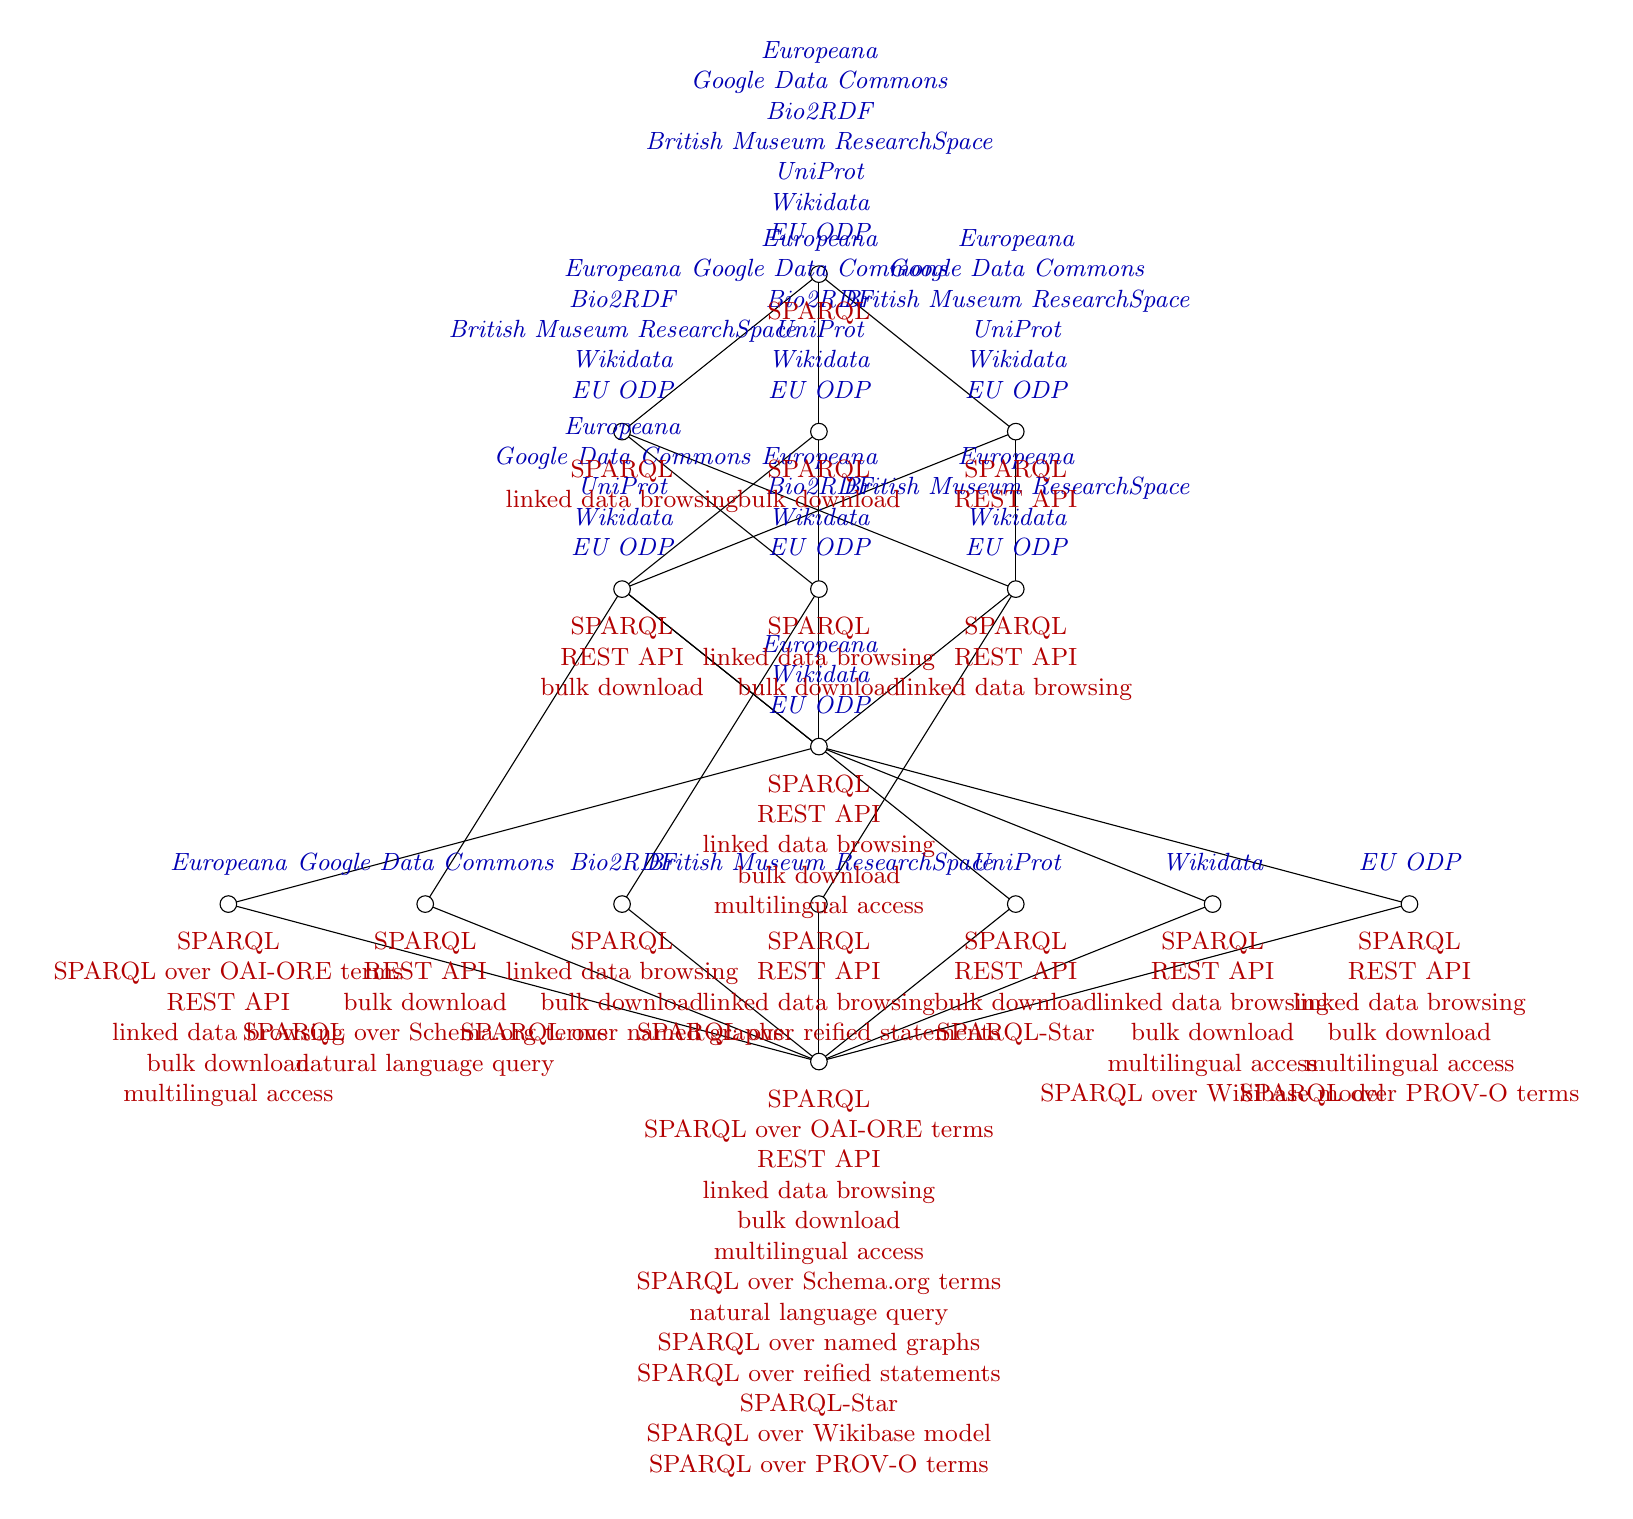
\begin{tikzpicture}[
    concept/.style={circle, draw, fill=white, inner sep=2pt, minimum size=6pt},
    lbl/.style={font=\small},
    obj/.style={font=\small\itshape, text=blue!70!black},
    attr/.style={font=\small, text=red!70!black}
]
  % Hasse edges
  \draw (0.000,0.000) -- (-7.500,2.000);
  \draw (0.000,0.000) -- (-5.000,2.000);
  \draw (0.000,0.000) -- (-2.500,2.000);
  \draw (0.000,0.000) -- (0.000,2.000);
  \draw (0.000,0.000) -- (2.500,2.000);
  \draw (0.000,0.000) -- (5.000,2.000);
  \draw (0.000,0.000) -- (7.500,2.000);
  \draw (-7.500,2.000) -- (0.000,4.000);
  \draw (-5.000,2.000) -- (-2.500,6.000);
  \draw (-2.500,2.000) -- (0.000,6.000);
  \draw (0.000,2.000) -- (2.500,6.000);
  \draw (2.500,2.000) -- (-2.500,6.000);
  \draw (5.000,2.000) -- (0.000,4.000);
  \draw (7.500,2.000) -- (0.000,4.000);
  \draw (0.000,4.000) -- (0.000,6.000);
  \draw (0.000,4.000) -- (2.500,6.000);
  \draw (0.000,4.000) -- (-2.500,6.000);
  \draw (0.000,6.000) -- (-2.500,8.000);
  \draw (0.000,6.000) -- (0.000,8.000);
  \draw (2.500,6.000) -- (-2.500,8.000);
  \draw (2.500,6.000) -- (2.500,8.000);
  \draw (-2.500,6.000) -- (0.000,8.000);
  \draw (-2.500,6.000) -- (2.500,8.000);
  \draw (-2.500,8.000) -- (0.000,10.000);
  \draw (0.000,8.000) -- (0.000,10.000);
  \draw (2.500,8.000) -- (0.000,10.000);
  % Concept nodes
  \node[concept] (n0) at (0.000,0.000) {};
  \node[concept] (n1) at (-7.500,2.000) {};
  \node[concept] (n2) at (-5.000,2.000) {};
  \node[concept] (n3) at (-2.500,2.000) {};
  \node[concept] (n4) at (0.000,2.000) {};
  \node[concept] (n5) at (2.500,2.000) {};
  \node[concept] (n6) at (5.000,2.000) {};
  \node[concept] (n7) at (7.500,2.000) {};
  \node[concept] (n8) at (0.000,4.000) {};
  \node[concept] (n9) at (0.000,6.000) {};
  \node[concept] (n10) at (2.500,6.000) {};
  \node[concept] (n11) at (-2.500,6.000) {};
  \node[concept] (n12) at (-2.500,8.000) {};
  \node[concept] (n13) at (0.000,8.000) {};
  \node[concept] (n14) at (2.500,8.000) {};
  \node[concept] (n15) at (0.000,10.000) {};
  % Object labels (above)
  \node[obj, above=2pt of n1, align=center] {\begin{tabular}{c}Europeana\end{tabular}};
  \node[obj, above=2pt of n2, align=center] {\begin{tabular}{c}Google Data Commons\end{tabular}};
  \node[obj, above=2pt of n3, align=center] {\begin{tabular}{c}Bio2RDF\end{tabular}};
  \node[obj, above=2pt of n4, align=center] {\begin{tabular}{c}British Museum ResearchSpace\end{tabular}};
  \node[obj, above=2pt of n5, align=center] {\begin{tabular}{c}UniProt\end{tabular}};
  \node[obj, above=2pt of n6, align=center] {\begin{tabular}{c}Wikidata\end{tabular}};
  \node[obj, above=2pt of n7, align=center] {\begin{tabular}{c}EU ODP\end{tabular}};
  \node[obj, above=2pt of n8, align=center] {\begin{tabular}{c}Europeana \\ Wikidata \\ EU ODP\end{tabular}};
  \node[obj, above=2pt of n9, align=center] {\begin{tabular}{c}Europeana \\ Bio2RDF \\ Wikidata \\ EU ODP\end{tabular}};
  \node[obj, above=2pt of n10, align=center] {\begin{tabular}{c}Europeana \\ British Museum ResearchSpace \\ Wikidata \\ EU ODP\end{tabular}};
  \node[obj, above=2pt of n11, align=center] {\begin{tabular}{c}Europeana \\ Google Data Commons \\ UniProt \\ Wikidata \\ EU ODP\end{tabular}};
  \node[obj, above=2pt of n12, align=center] {\begin{tabular}{c}Europeana \\ Bio2RDF \\ British Museum ResearchSpace \\ Wikidata \\ EU ODP\end{tabular}};
  \node[obj, above=2pt of n13, align=center] {\begin{tabular}{c}Europeana \\ Google Data Commons \\ Bio2RDF \\ UniProt \\ Wikidata \\ EU ODP\end{tabular}};
  \node[obj, above=2pt of n14, align=center] {\begin{tabular}{c}Europeana \\ Google Data Commons \\ British Museum ResearchSpace \\ UniProt \\ Wikidata \\ EU ODP\end{tabular}};
  \node[obj, above=2pt of n15, align=center] {\begin{tabular}{c}Europeana \\ Google Data Commons \\ Bio2RDF \\ British Museum ResearchSpace \\ UniProt \\ Wikidata \\ EU ODP\end{tabular}};
  % Attribute labels (below)
  \node[attr, below=2pt of n0, align=center] {\begin{tabular}{c}SPARQL \\ SPARQL over OAI-ORE terms \\ REST API \\ linked data browsing \\ bulk download \\ multilingual access \\ SPARQL over Schema.org terms \\ natural language query \\ SPARQL over named graphs \\ SPARQL over reified statements \\ SPARQL-Star \\ SPARQL over Wikibase model \\ SPARQL over PROV-O terms\end{tabular}};
  \node[attr, below=2pt of n1, align=center] {\begin{tabular}{c}SPARQL \\ SPARQL over OAI-ORE terms \\ REST API \\ linked data browsing \\ bulk download \\ multilingual access\end{tabular}};
  \node[attr, below=2pt of n2, align=center] {\begin{tabular}{c}SPARQL \\ REST API \\ bulk download \\ SPARQL over Schema.org terms \\ natural language query\end{tabular}};
  \node[attr, below=2pt of n3, align=center] {\begin{tabular}{c}SPARQL \\ linked data browsing \\ bulk download \\ SPARQL over named graphs\end{tabular}};
  \node[attr, below=2pt of n4, align=center] {\begin{tabular}{c}SPARQL \\ REST API \\ linked data browsing \\ SPARQL over reified statements\end{tabular}};
  \node[attr, below=2pt of n5, align=center] {\begin{tabular}{c}SPARQL \\ REST API \\ bulk download \\ SPARQL-Star\end{tabular}};
  \node[attr, below=2pt of n6, align=center] {\begin{tabular}{c}SPARQL \\ REST API \\ linked data browsing \\ bulk download \\ multilingual access \\ SPARQL over Wikibase model\end{tabular}};
  \node[attr, below=2pt of n7, align=center] {\begin{tabular}{c}SPARQL \\ REST API \\ linked data browsing \\ bulk download \\ multilingual access \\ SPARQL over PROV-O terms\end{tabular}};
  \node[attr, below=2pt of n8, align=center] {\begin{tabular}{c}SPARQL \\ REST API \\ linked data browsing \\ bulk download \\ multilingual access\end{tabular}};
  \node[attr, below=2pt of n9, align=center] {\begin{tabular}{c}SPARQL \\ linked data browsing \\ bulk download\end{tabular}};
  \node[attr, below=2pt of n10, align=center] {\begin{tabular}{c}SPARQL \\ REST API \\ linked data browsing\end{tabular}};
  \node[attr, below=2pt of n11, align=center] {\begin{tabular}{c}SPARQL \\ REST API \\ bulk download\end{tabular}};
  \node[attr, below=2pt of n12, align=center] {\begin{tabular}{c}SPARQL \\ linked data browsing\end{tabular}};
  \node[attr, below=2pt of n13, align=center] {\begin{tabular}{c}SPARQL \\ bulk download\end{tabular}};
  \node[attr, below=2pt of n14, align=center] {\begin{tabular}{c}SPARQL \\ REST API\end{tabular}};
  \node[attr, below=2pt of n15, align=center] {\begin{tabular}{c}SPARQL\end{tabular}};
\end{tikzpicture}
  \caption{FCA lattice: pragmatic affordances}
  \label{fig:fca-pragmatic_affordances}
\end{figure}

% ────────────────────────────────────────────────────────────
% pragmatic properties
% ────────────────────────────────────────────────────────────
\begin{figure}[htbp]
  \centering
  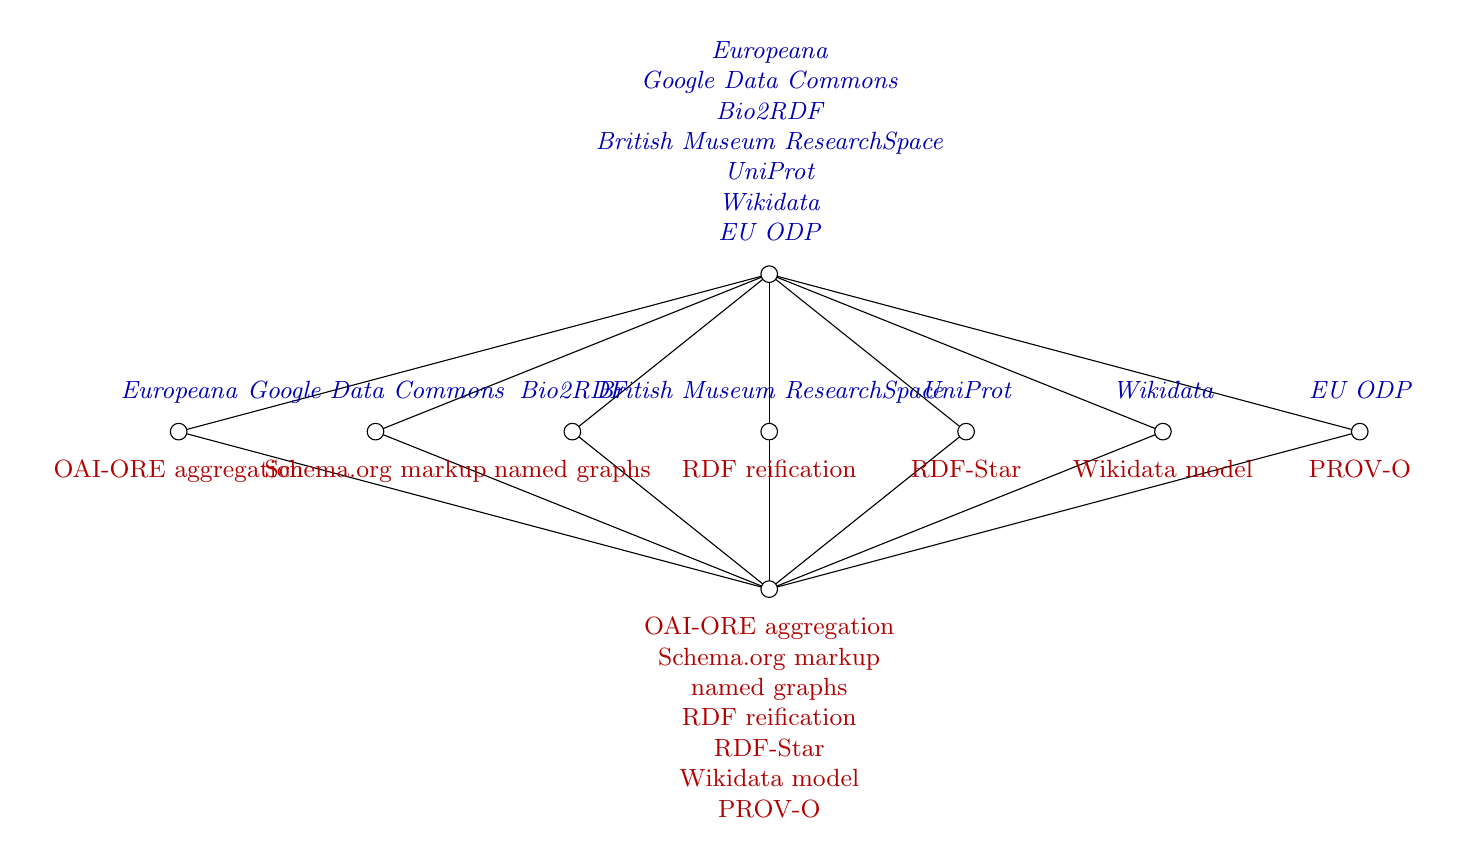
\begin{tikzpicture}[
    concept/.style={circle, draw, fill=white, inner sep=2pt, minimum size=6pt},
    lbl/.style={font=\small},
    obj/.style={font=\small\itshape, text=blue!70!black},
    attr/.style={font=\small, text=red!70!black}
]
  % Hasse edges
  \draw (0.000,0.000) -- (-7.500,2.000);
  \draw (0.000,0.000) -- (-5.000,2.000);
  \draw (0.000,0.000) -- (-2.500,2.000);
  \draw (0.000,0.000) -- (0.000,2.000);
  \draw (0.000,0.000) -- (2.500,2.000);
  \draw (0.000,0.000) -- (5.000,2.000);
  \draw (0.000,0.000) -- (7.500,2.000);
  \draw (-7.500,2.000) -- (0.000,4.000);
  \draw (-5.000,2.000) -- (0.000,4.000);
  \draw (-2.500,2.000) -- (0.000,4.000);
  \draw (0.000,2.000) -- (0.000,4.000);
  \draw (2.500,2.000) -- (0.000,4.000);
  \draw (5.000,2.000) -- (0.000,4.000);
  \draw (7.500,2.000) -- (0.000,4.000);
  % Concept nodes
  \node[concept] (n0) at (0.000,0.000) {};
  \node[concept] (n1) at (-7.500,2.000) {};
  \node[concept] (n2) at (-5.000,2.000) {};
  \node[concept] (n3) at (-2.500,2.000) {};
  \node[concept] (n4) at (0.000,2.000) {};
  \node[concept] (n5) at (2.500,2.000) {};
  \node[concept] (n6) at (5.000,2.000) {};
  \node[concept] (n7) at (7.500,2.000) {};
  \node[concept] (n8) at (0.000,4.000) {};
  % Object labels (above)
  \node[obj, above=2pt of n1, align=center] {\begin{tabular}{c}Europeana\end{tabular}};
  \node[obj, above=2pt of n2, align=center] {\begin{tabular}{c}Google Data Commons\end{tabular}};
  \node[obj, above=2pt of n3, align=center] {\begin{tabular}{c}Bio2RDF\end{tabular}};
  \node[obj, above=2pt of n4, align=center] {\begin{tabular}{c}British Museum ResearchSpace\end{tabular}};
  \node[obj, above=2pt of n5, align=center] {\begin{tabular}{c}UniProt\end{tabular}};
  \node[obj, above=2pt of n6, align=center] {\begin{tabular}{c}Wikidata\end{tabular}};
  \node[obj, above=2pt of n7, align=center] {\begin{tabular}{c}EU ODP\end{tabular}};
  \node[obj, above=2pt of n8, align=center] {\begin{tabular}{c}Europeana \\ Google Data Commons \\ Bio2RDF \\ British Museum ResearchSpace \\ UniProt \\ Wikidata \\ EU ODP\end{tabular}};
  % Attribute labels (below)
  \node[attr, below=2pt of n0, align=center] {\begin{tabular}{c}OAI-ORE aggregation \\ Schema.org markup \\ named graphs \\ RDF reification \\ RDF-Star \\ Wikidata model \\ PROV-O\end{tabular}};
  \node[attr, below=2pt of n1, align=center] {\begin{tabular}{c}OAI-ORE aggregation\end{tabular}};
  \node[attr, below=2pt of n2, align=center] {\begin{tabular}{c}Schema.org markup\end{tabular}};
  \node[attr, below=2pt of n3, align=center] {\begin{tabular}{c}named graphs\end{tabular}};
  \node[attr, below=2pt of n4, align=center] {\begin{tabular}{c}RDF reification\end{tabular}};
  \node[attr, below=2pt of n5, align=center] {\begin{tabular}{c}RDF-Star\end{tabular}};
  \node[attr, below=2pt of n6, align=center] {\begin{tabular}{c}Wikidata model\end{tabular}};
  \node[attr, below=2pt of n7, align=center] {\begin{tabular}{c}PROV-O\end{tabular}};
\end{tikzpicture}
  \caption{FCA lattice: pragmatic properties}
  \label{fig:fca-pragmatic_properties}
\end{figure}

% ────────────────────────────────────────────────────────────
% semantic affordances
% ────────────────────────────────────────────────────────────
\begin{figure}[htbp]
  \centering
  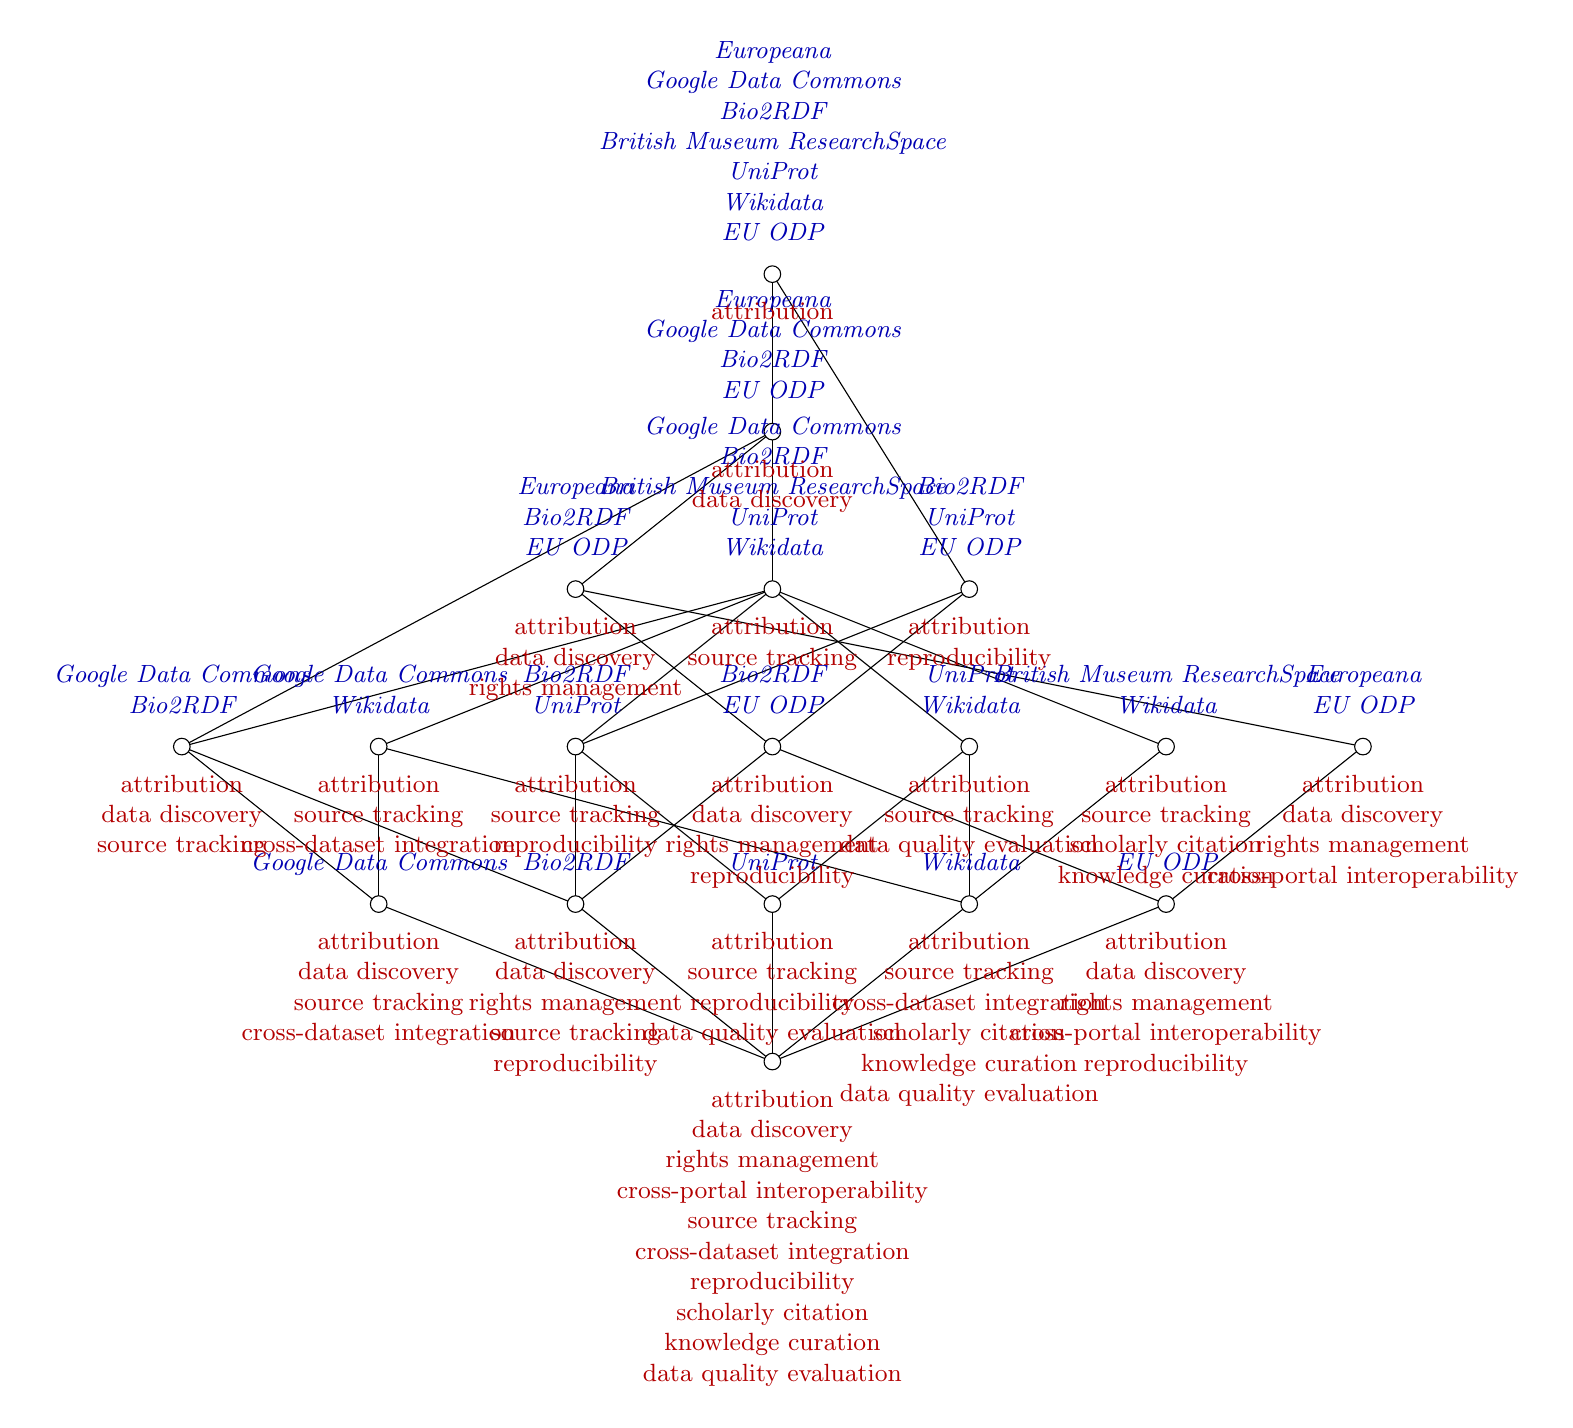
\begin{tikzpicture}[
    concept/.style={circle, draw, fill=white, inner sep=2pt, minimum size=6pt},
    lbl/.style={font=\small},
    obj/.style={font=\small\itshape, text=blue!70!black},
    attr/.style={font=\small, text=red!70!black}
]
  % Hasse edges
  \draw (0.000,0.000) -- (-5.000,2.000);
  \draw (0.000,0.000) -- (-2.500,2.000);
  \draw (0.000,0.000) -- (0.000,2.000);
  \draw (0.000,0.000) -- (2.500,2.000);
  \draw (0.000,0.000) -- (5.000,2.000);
  \draw (-5.000,2.000) -- (-7.500,4.000);
  \draw (-5.000,2.000) -- (-5.000,4.000);
  \draw (-2.500,2.000) -- (-7.500,4.000);
  \draw (-2.500,2.000) -- (-2.500,4.000);
  \draw (-2.500,2.000) -- (0.000,4.000);
  \draw (0.000,2.000) -- (-2.500,4.000);
  \draw (0.000,2.000) -- (2.500,4.000);
  \draw (2.500,2.000) -- (-5.000,4.000);
  \draw (2.500,2.000) -- (5.000,4.000);
  \draw (2.500,2.000) -- (2.500,4.000);
  \draw (5.000,2.000) -- (7.500,4.000);
  \draw (5.000,2.000) -- (0.000,4.000);
  \draw (7.500,4.000) -- (-2.500,6.000);
  \draw (-7.500,4.000) -- (0.000,8.000);
  \draw (-7.500,4.000) -- (0.000,6.000);
  \draw (-5.000,4.000) -- (0.000,6.000);
  \draw (-2.500,4.000) -- (2.500,6.000);
  \draw (-2.500,4.000) -- (0.000,6.000);
  \draw (0.000,4.000) -- (-2.500,6.000);
  \draw (0.000,4.000) -- (2.500,6.000);
  \draw (5.000,4.000) -- (0.000,6.000);
  \draw (2.500,4.000) -- (0.000,6.000);
  \draw (-2.500,6.000) -- (0.000,8.000);
  \draw (2.500,6.000) -- (0.000,10.000);
  \draw (0.000,8.000) -- (0.000,10.000);
  \draw (0.000,6.000) -- (0.000,10.000);
  % Concept nodes
  \node[concept] (n0) at (0.000,0.000) {};
  \node[concept] (n1) at (-5.000,2.000) {};
  \node[concept] (n2) at (-2.500,2.000) {};
  \node[concept] (n3) at (0.000,2.000) {};
  \node[concept] (n4) at (2.500,2.000) {};
  \node[concept] (n5) at (5.000,2.000) {};
  \node[concept] (n6) at (7.500,4.000) {};
  \node[concept] (n7) at (-7.500,4.000) {};
  \node[concept] (n8) at (-5.000,4.000) {};
  \node[concept] (n9) at (-2.500,4.000) {};
  \node[concept] (n10) at (0.000,4.000) {};
  \node[concept] (n11) at (5.000,4.000) {};
  \node[concept] (n12) at (2.500,4.000) {};
  \node[concept] (n13) at (-2.500,6.000) {};
  \node[concept] (n14) at (2.500,6.000) {};
  \node[concept] (n15) at (0.000,8.000) {};
  \node[concept] (n16) at (0.000,6.000) {};
  \node[concept] (n17) at (0.000,10.000) {};
  % Object labels (above)
  \node[obj, above=2pt of n1, align=center] {\begin{tabular}{c}Google Data Commons\end{tabular}};
  \node[obj, above=2pt of n2, align=center] {\begin{tabular}{c}Bio2RDF\end{tabular}};
  \node[obj, above=2pt of n3, align=center] {\begin{tabular}{c}UniProt\end{tabular}};
  \node[obj, above=2pt of n4, align=center] {\begin{tabular}{c}Wikidata\end{tabular}};
  \node[obj, above=2pt of n5, align=center] {\begin{tabular}{c}EU ODP\end{tabular}};
  \node[obj, above=2pt of n6, align=center] {\begin{tabular}{c}Europeana \\ EU ODP\end{tabular}};
  \node[obj, above=2pt of n7, align=center] {\begin{tabular}{c}Google Data Commons \\ Bio2RDF\end{tabular}};
  \node[obj, above=2pt of n8, align=center] {\begin{tabular}{c}Google Data Commons \\ Wikidata\end{tabular}};
  \node[obj, above=2pt of n9, align=center] {\begin{tabular}{c}Bio2RDF \\ UniProt\end{tabular}};
  \node[obj, above=2pt of n10, align=center] {\begin{tabular}{c}Bio2RDF \\ EU ODP\end{tabular}};
  \node[obj, above=2pt of n11, align=center] {\begin{tabular}{c}British Museum ResearchSpace \\ Wikidata\end{tabular}};
  \node[obj, above=2pt of n12, align=center] {\begin{tabular}{c}UniProt \\ Wikidata\end{tabular}};
  \node[obj, above=2pt of n13, align=center] {\begin{tabular}{c}Europeana \\ Bio2RDF \\ EU ODP\end{tabular}};
  \node[obj, above=2pt of n14, align=center] {\begin{tabular}{c}Bio2RDF \\ UniProt \\ EU ODP\end{tabular}};
  \node[obj, above=2pt of n15, align=center] {\begin{tabular}{c}Europeana \\ Google Data Commons \\ Bio2RDF \\ EU ODP\end{tabular}};
  \node[obj, above=2pt of n16, align=center] {\begin{tabular}{c}Google Data Commons \\ Bio2RDF \\ British Museum ResearchSpace \\ UniProt \\ Wikidata\end{tabular}};
  \node[obj, above=2pt of n17, align=center] {\begin{tabular}{c}Europeana \\ Google Data Commons \\ Bio2RDF \\ British Museum ResearchSpace \\ UniProt \\ Wikidata \\ EU ODP\end{tabular}};
  % Attribute labels (below)
  \node[attr, below=2pt of n0, align=center] {\begin{tabular}{c}attribution \\ data discovery \\ rights management \\ cross-portal interoperability \\ source tracking \\ cross-dataset integration \\ reproducibility \\ scholarly citation \\ knowledge curation \\ data quality evaluation\end{tabular}};
  \node[attr, below=2pt of n1, align=center] {\begin{tabular}{c}attribution \\ data discovery \\ source tracking \\ cross-dataset integration\end{tabular}};
  \node[attr, below=2pt of n2, align=center] {\begin{tabular}{c}attribution \\ data discovery \\ rights management \\ source tracking \\ reproducibility\end{tabular}};
  \node[attr, below=2pt of n3, align=center] {\begin{tabular}{c}attribution \\ source tracking \\ reproducibility \\ data quality evaluation\end{tabular}};
  \node[attr, below=2pt of n4, align=center] {\begin{tabular}{c}attribution \\ source tracking \\ cross-dataset integration \\ scholarly citation \\ knowledge curation \\ data quality evaluation\end{tabular}};
  \node[attr, below=2pt of n5, align=center] {\begin{tabular}{c}attribution \\ data discovery \\ rights management \\ cross-portal interoperability \\ reproducibility\end{tabular}};
  \node[attr, below=2pt of n6, align=center] {\begin{tabular}{c}attribution \\ data discovery \\ rights management \\ cross-portal interoperability\end{tabular}};
  \node[attr, below=2pt of n7, align=center] {\begin{tabular}{c}attribution \\ data discovery \\ source tracking\end{tabular}};
  \node[attr, below=2pt of n8, align=center] {\begin{tabular}{c}attribution \\ source tracking \\ cross-dataset integration\end{tabular}};
  \node[attr, below=2pt of n9, align=center] {\begin{tabular}{c}attribution \\ source tracking \\ reproducibility\end{tabular}};
  \node[attr, below=2pt of n10, align=center] {\begin{tabular}{c}attribution \\ data discovery \\ rights management \\ reproducibility\end{tabular}};
  \node[attr, below=2pt of n11, align=center] {\begin{tabular}{c}attribution \\ source tracking \\ scholarly citation \\ knowledge curation\end{tabular}};
  \node[attr, below=2pt of n12, align=center] {\begin{tabular}{c}attribution \\ source tracking \\ data quality evaluation\end{tabular}};
  \node[attr, below=2pt of n13, align=center] {\begin{tabular}{c}attribution \\ data discovery \\ rights management\end{tabular}};
  \node[attr, below=2pt of n14, align=center] {\begin{tabular}{c}attribution \\ reproducibility\end{tabular}};
  \node[attr, below=2pt of n15, align=center] {\begin{tabular}{c}attribution \\ data discovery\end{tabular}};
  \node[attr, below=2pt of n16, align=center] {\begin{tabular}{c}attribution \\ source tracking\end{tabular}};
  \node[attr, below=2pt of n17, align=center] {\begin{tabular}{c}attribution\end{tabular}};
\end{tikzpicture}
  \caption{FCA lattice: semantic affordances}
  \label{fig:fca-semantic_affordances}
\end{figure}

% ────────────────────────────────────────────────────────────
% semantic properties
% ────────────────────────────────────────────────────────────
\begin{figure}[htbp]
  \centering
  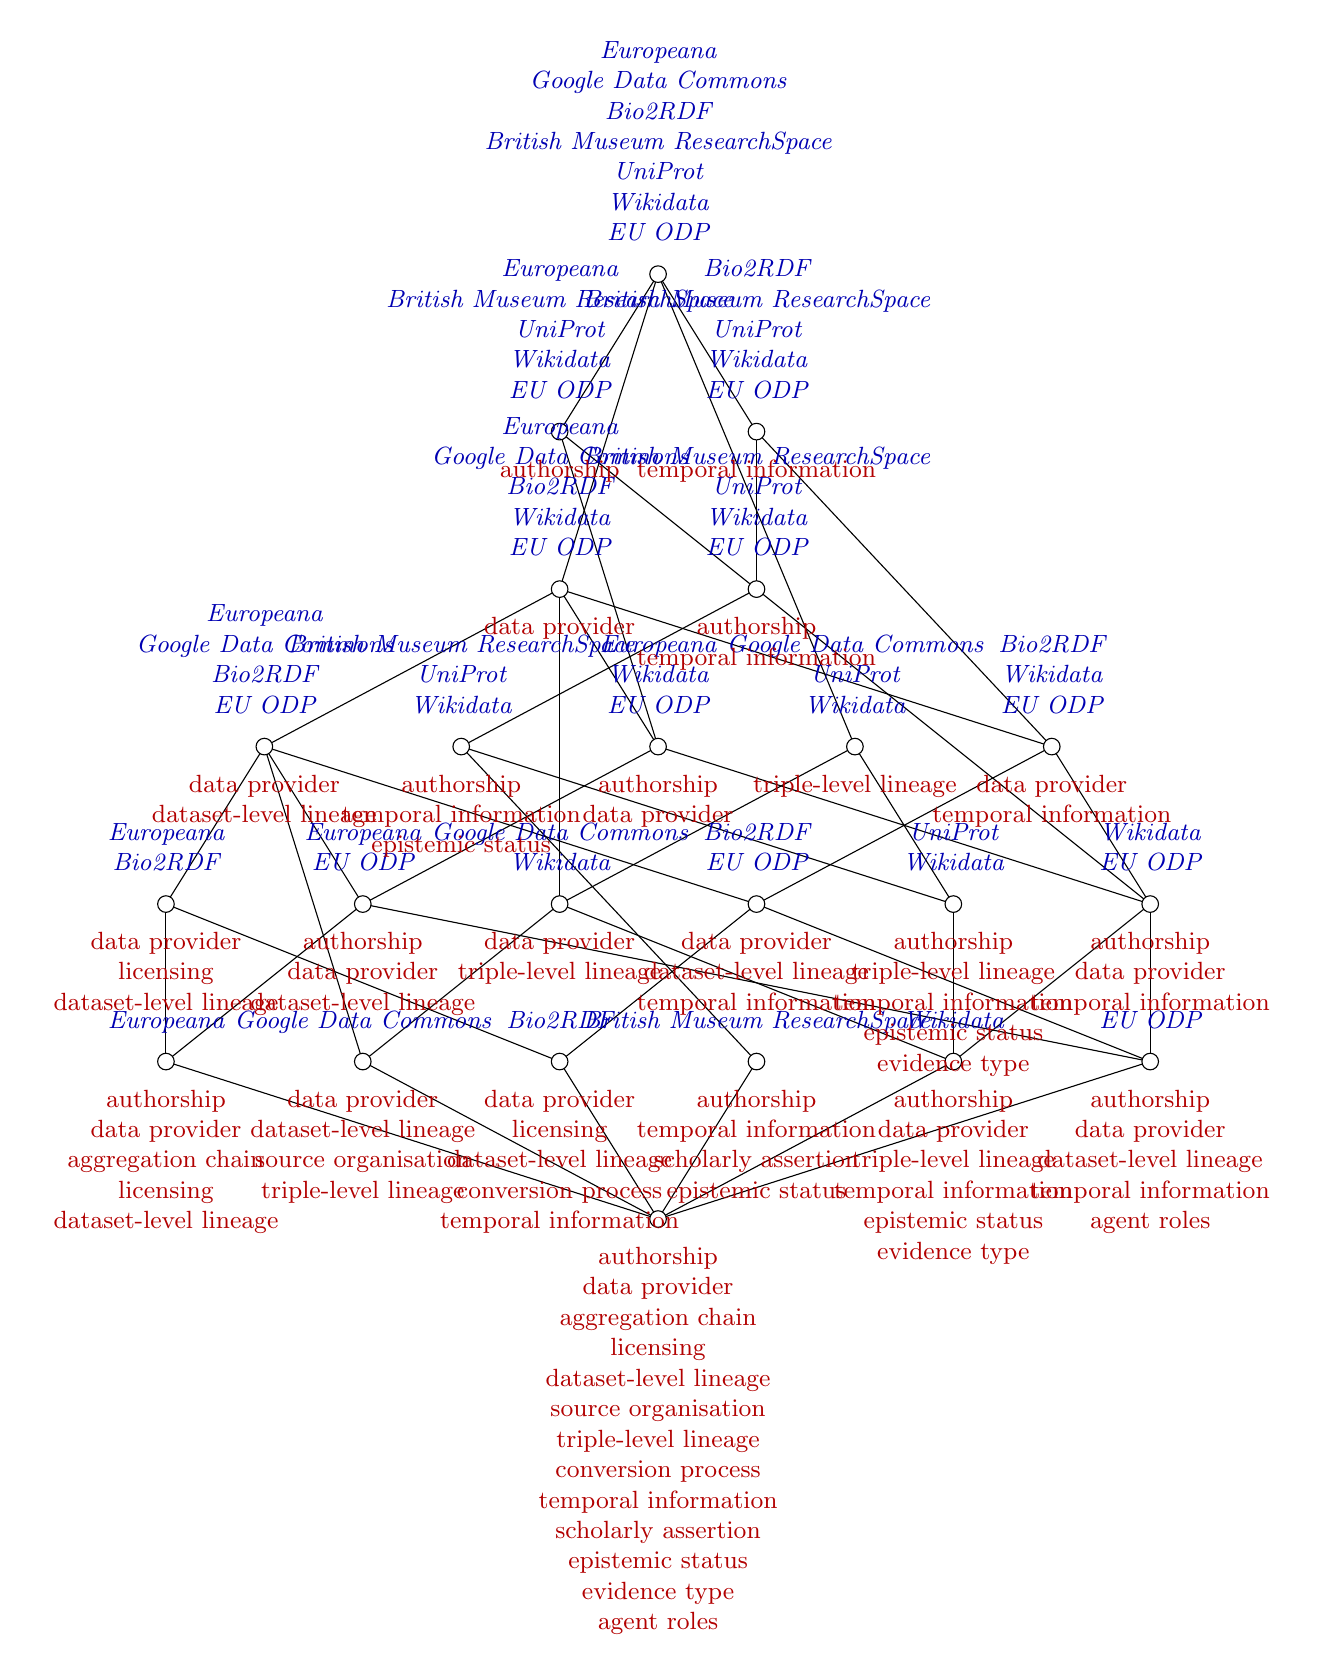
\begin{tikzpicture}[
    concept/.style={circle, draw, fill=white, inner sep=2pt, minimum size=6pt},
    lbl/.style={font=\small},
    obj/.style={font=\small\itshape, text=blue!70!black},
    attr/.style={font=\small, text=red!70!black}
]
  % Hasse edges
  \draw (0.000,0.000) -- (-6.250,2.000);
  \draw (0.000,0.000) -- (-3.750,2.000);
  \draw (0.000,0.000) -- (-1.250,2.000);
  \draw (0.000,0.000) -- (1.250,2.000);
  \draw (0.000,0.000) -- (3.750,2.000);
  \draw (0.000,0.000) -- (6.250,2.000);
  \draw (-6.250,2.000) -- (-6.250,4.000);
  \draw (-6.250,2.000) -- (-3.750,4.000);
  \draw (-3.750,2.000) -- (-1.250,4.000);
  \draw (-3.750,2.000) -- (-5.000,6.000);
  \draw (-1.250,2.000) -- (-6.250,4.000);
  \draw (-1.250,2.000) -- (1.250,4.000);
  \draw (1.250,2.000) -- (-2.500,6.000);
  \draw (3.750,2.000) -- (-1.250,4.000);
  \draw (3.750,2.000) -- (3.750,4.000);
  \draw (3.750,2.000) -- (6.250,4.000);
  \draw (6.250,2.000) -- (-3.750,4.000);
  \draw (6.250,2.000) -- (1.250,4.000);
  \draw (6.250,2.000) -- (6.250,4.000);
  \draw (-6.250,4.000) -- (-5.000,6.000);
  \draw (-3.750,4.000) -- (0.000,6.000);
  \draw (-3.750,4.000) -- (-5.000,6.000);
  \draw (-1.250,4.000) -- (2.500,6.000);
  \draw (-1.250,4.000) -- (-1.250,8.000);
  \draw (1.250,4.000) -- (5.000,6.000);
  \draw (1.250,4.000) -- (-5.000,6.000);
  \draw (3.750,4.000) -- (2.500,6.000);
  \draw (3.750,4.000) -- (-2.500,6.000);
  \draw (6.250,4.000) -- (0.000,6.000);
  \draw (6.250,4.000) -- (5.000,6.000);
  \draw (6.250,4.000) -- (1.250,8.000);
  \draw (0.000,6.000) -- (-1.250,8.000);
  \draw (0.000,6.000) -- (-1.250,10.000);
  \draw (2.500,6.000) -- (0.000,12.000);
  \draw (5.000,6.000) -- (-1.250,8.000);
  \draw (5.000,6.000) -- (1.250,10.000);
  \draw (-2.500,6.000) -- (1.250,8.000);
  \draw (-5.000,6.000) -- (-1.250,8.000);
  \draw (1.250,8.000) -- (-1.250,10.000);
  \draw (1.250,8.000) -- (1.250,10.000);
  \draw (-1.250,8.000) -- (0.000,12.000);
  \draw (-1.250,10.000) -- (0.000,12.000);
  \draw (1.250,10.000) -- (0.000,12.000);
  % Concept nodes
  \node[concept] (n0) at (0.000,0.000) {};
  \node[concept] (n1) at (-6.250,2.000) {};
  \node[concept] (n2) at (-3.750,2.000) {};
  \node[concept] (n3) at (-1.250,2.000) {};
  \node[concept] (n4) at (1.250,2.000) {};
  \node[concept] (n5) at (3.750,2.000) {};
  \node[concept] (n6) at (6.250,2.000) {};
  \node[concept] (n7) at (-6.250,4.000) {};
  \node[concept] (n8) at (-3.750,4.000) {};
  \node[concept] (n9) at (-1.250,4.000) {};
  \node[concept] (n10) at (1.250,4.000) {};
  \node[concept] (n11) at (3.750,4.000) {};
  \node[concept] (n12) at (6.250,4.000) {};
  \node[concept] (n13) at (0.000,6.000) {};
  \node[concept] (n14) at (2.500,6.000) {};
  \node[concept] (n15) at (5.000,6.000) {};
  \node[concept] (n16) at (-2.500,6.000) {};
  \node[concept] (n17) at (-5.000,6.000) {};
  \node[concept] (n18) at (1.250,8.000) {};
  \node[concept] (n19) at (-1.250,8.000) {};
  \node[concept] (n20) at (-1.250,10.000) {};
  \node[concept] (n21) at (1.250,10.000) {};
  \node[concept] (n22) at (0.000,12.000) {};
  % Object labels (above)
  \node[obj, above=2pt of n1, align=center] {\begin{tabular}{c}Europeana\end{tabular}};
  \node[obj, above=2pt of n2, align=center] {\begin{tabular}{c}Google Data Commons\end{tabular}};
  \node[obj, above=2pt of n3, align=center] {\begin{tabular}{c}Bio2RDF\end{tabular}};
  \node[obj, above=2pt of n4, align=center] {\begin{tabular}{c}British Museum ResearchSpace\end{tabular}};
  \node[obj, above=2pt of n5, align=center] {\begin{tabular}{c}Wikidata\end{tabular}};
  \node[obj, above=2pt of n6, align=center] {\begin{tabular}{c}EU ODP\end{tabular}};
  \node[obj, above=2pt of n7, align=center] {\begin{tabular}{c}Europeana \\ Bio2RDF\end{tabular}};
  \node[obj, above=2pt of n8, align=center] {\begin{tabular}{c}Europeana \\ EU ODP\end{tabular}};
  \node[obj, above=2pt of n9, align=center] {\begin{tabular}{c}Google Data Commons \\ Wikidata\end{tabular}};
  \node[obj, above=2pt of n10, align=center] {\begin{tabular}{c}Bio2RDF \\ EU ODP\end{tabular}};
  \node[obj, above=2pt of n11, align=center] {\begin{tabular}{c}UniProt \\ Wikidata\end{tabular}};
  \node[obj, above=2pt of n12, align=center] {\begin{tabular}{c}Wikidata \\ EU ODP\end{tabular}};
  \node[obj, above=2pt of n13, align=center] {\begin{tabular}{c}Europeana \\ Wikidata \\ EU ODP\end{tabular}};
  \node[obj, above=2pt of n14, align=center] {\begin{tabular}{c}Google Data Commons \\ UniProt \\ Wikidata\end{tabular}};
  \node[obj, above=2pt of n15, align=center] {\begin{tabular}{c}Bio2RDF \\ Wikidata \\ EU ODP\end{tabular}};
  \node[obj, above=2pt of n16, align=center] {\begin{tabular}{c}British Museum ResearchSpace \\ UniProt \\ Wikidata\end{tabular}};
  \node[obj, above=2pt of n17, align=center] {\begin{tabular}{c}Europeana \\ Google Data Commons \\ Bio2RDF \\ EU ODP\end{tabular}};
  \node[obj, above=2pt of n18, align=center] {\begin{tabular}{c}British Museum ResearchSpace \\ UniProt \\ Wikidata \\ EU ODP\end{tabular}};
  \node[obj, above=2pt of n19, align=center] {\begin{tabular}{c}Europeana \\ Google Data Commons \\ Bio2RDF \\ Wikidata \\ EU ODP\end{tabular}};
  \node[obj, above=2pt of n20, align=center] {\begin{tabular}{c}Europeana \\ British Museum ResearchSpace \\ UniProt \\ Wikidata \\ EU ODP\end{tabular}};
  \node[obj, above=2pt of n21, align=center] {\begin{tabular}{c}Bio2RDF \\ British Museum ResearchSpace \\ UniProt \\ Wikidata \\ EU ODP\end{tabular}};
  \node[obj, above=2pt of n22, align=center] {\begin{tabular}{c}Europeana \\ Google Data Commons \\ Bio2RDF \\ British Museum ResearchSpace \\ UniProt \\ Wikidata \\ EU ODP\end{tabular}};
  % Attribute labels (below)
  \node[attr, below=2pt of n0, align=center] {\begin{tabular}{c}authorship \\ data provider \\ aggregation chain \\ licensing \\ dataset-level lineage \\ source organisation \\ triple-level lineage \\ conversion process \\ temporal information \\ scholarly assertion \\ epistemic status \\ evidence type \\ agent roles\end{tabular}};
  \node[attr, below=2pt of n1, align=center] {\begin{tabular}{c}authorship \\ data provider \\ aggregation chain \\ licensing \\ dataset-level lineage\end{tabular}};
  \node[attr, below=2pt of n2, align=center] {\begin{tabular}{c}data provider \\ dataset-level lineage \\ source organisation \\ triple-level lineage\end{tabular}};
  \node[attr, below=2pt of n3, align=center] {\begin{tabular}{c}data provider \\ licensing \\ dataset-level lineage \\ conversion process \\ temporal information\end{tabular}};
  \node[attr, below=2pt of n4, align=center] {\begin{tabular}{c}authorship \\ temporal information \\ scholarly assertion \\ epistemic status\end{tabular}};
  \node[attr, below=2pt of n5, align=center] {\begin{tabular}{c}authorship \\ data provider \\ triple-level lineage \\ temporal information \\ epistemic status \\ evidence type\end{tabular}};
  \node[attr, below=2pt of n6, align=center] {\begin{tabular}{c}authorship \\ data provider \\ dataset-level lineage \\ temporal information \\ agent roles\end{tabular}};
  \node[attr, below=2pt of n7, align=center] {\begin{tabular}{c}data provider \\ licensing \\ dataset-level lineage\end{tabular}};
  \node[attr, below=2pt of n8, align=center] {\begin{tabular}{c}authorship \\ data provider \\ dataset-level lineage\end{tabular}};
  \node[attr, below=2pt of n9, align=center] {\begin{tabular}{c}data provider \\ triple-level lineage\end{tabular}};
  \node[attr, below=2pt of n10, align=center] {\begin{tabular}{c}data provider \\ dataset-level lineage \\ temporal information\end{tabular}};
  \node[attr, below=2pt of n11, align=center] {\begin{tabular}{c}authorship \\ triple-level lineage \\ temporal information \\ epistemic status \\ evidence type\end{tabular}};
  \node[attr, below=2pt of n12, align=center] {\begin{tabular}{c}authorship \\ data provider \\ temporal information\end{tabular}};
  \node[attr, below=2pt of n13, align=center] {\begin{tabular}{c}authorship \\ data provider\end{tabular}};
  \node[attr, below=2pt of n14, align=center] {\begin{tabular}{c}triple-level lineage\end{tabular}};
  \node[attr, below=2pt of n15, align=center] {\begin{tabular}{c}data provider \\ temporal information\end{tabular}};
  \node[attr, below=2pt of n16, align=center] {\begin{tabular}{c}authorship \\ temporal information \\ epistemic status\end{tabular}};
  \node[attr, below=2pt of n17, align=center] {\begin{tabular}{c}data provider \\ dataset-level lineage\end{tabular}};
  \node[attr, below=2pt of n18, align=center] {\begin{tabular}{c}authorship \\ temporal information\end{tabular}};
  \node[attr, below=2pt of n19, align=center] {\begin{tabular}{c}data provider\end{tabular}};
  \node[attr, below=2pt of n20, align=center] {\begin{tabular}{c}authorship\end{tabular}};
  \node[attr, below=2pt of n21, align=center] {\begin{tabular}{c}temporal information\end{tabular}};
\end{tikzpicture}
  \caption{FCA lattice: semantic properties}
  \label{fig:fca-semantic_properties}
\end{figure}


\end{document}
